% =============================================================================
% PART III: COMPLETE CHRONOLOGY OF THE PROJECT
% =============================================================================

% -----------------------------------------------------------------------------
\section{How to Read This Part}
\label{sec:chr_intro}
% -----------------------------------------------------------------------------

Parts~\ref{part:mid} and~\ref{part:post} present the designs and the results. This part tells the same project as it actually happened, in time order, including the steps that did not work. For every stage we record what was tried, what was observed, what we concluded, and what was done next. Several conclusions that we reached on the way were later shown to be wrong, and we keep them here because they explain why the work took the path it did.

The project ran in two halves. The first half, up to the mid-review, built the L2 TLB designs in SE mode. The second half moved everything to full-system simulation. From 15 November onward two full-system campaigns ran in parallel on the department lab machines:
\begin{itemize}
    \item \textbf{The full-run campaign} ran each of five designs (Inclusive, Exclusive, NINE, Agile and Perforated Pages) as a \emph{lane}. In a lane, the guest boots on the atomic CPU and then runs every SPEC benchmark from start to end on the timing CPU. This campaign found and fixed most of the simulator problems described in this part.
    \item \textbf{The windowed campaign} ran all six designs, including CoLT-FA, with one \texttt{gem5} process per benchmark. Each benchmark runs on the atomic CPU, except for a measurement window on the timing CPU. This campaign produced the pass/fail matrix of Section~\ref{sec:fs_spec} and all the performance numbers of Part~\ref{part:post}.
\end{itemize}

Figure~\ref{fig:chr_journey} gives the overall path of the project and Figure~\ref{fig:chr_gantt} places the second-half activities on a calendar. Table~\ref{tab:chr_ledger} at the end of this part lists every problem in one place.

\begin{figure}[htbp]
\centering
\begin{tikzpicture}[
  node distance=0.35cm and 0.35cm,
  st/.style={draw, rounded corners, fill=#1, minimum width=2.6cm, minimum height=1.05cm, align=center, font=\scriptsize, text width=2.5cm},
  st/.default=blue!8,
  arr/.style={-{Stealth[length=2mm]}, thick}]
\node[st=gray!12] (a) {\textbf{SE designs}\\set-associative L2,\\inclusion policies};
\node[st=gray!12, right=of a] (b) {\textbf{SE mechanisms}\\prefetchers, CoLT-FA,\\Perforated, Hybrid};
\node[st=yellow!25, right=of b] (c) {\textbf{Mid-review}\\results in SE mode\\on microbenchmarks};
\node[st=orange!15, right=of c] (d) {\textbf{Audit and fix}\\six designs,\\\texttt{.fixed} files};
\node[st=green!12, below=0.8cm of d] (e) {\textbf{Verify in SE}\\translation oracle,\\invariant checkers};
\node[st=blue!10, left=of e] (f) {\textbf{Full-system bring-up}\\Ubuntu guest,\\SPEC disk, scripts};
\node[st=blue!10, left=of f] (g) {\textbf{Two campaigns}\\full-run lanes and\\windowed shards};
\node[st=red!10, left=of g] (h) {\textbf{Simulator bugs}\\i8237, walker,\\memory map, x87};
\node[st=purple!10, below=0.8cm of h] (i) {\textbf{TLB workloads}\\GAPBS, memcached,\\XSBench, SPEC ref};
\node[st=purple!10, right=of i] (j) {\textbf{Second looks}\\Perforated strict,\\same-host rule};
\node[st=yellow!25, right=of j] (k) {\textbf{Final results}\\report, artifact,\\presentation};
\draw[arr] (a) -- (b); \draw[arr] (b) -- (c); \draw[arr] (c) -- (d);
\draw[arr] (d) -- (e); \draw[arr] (e) -- (f); \draw[arr] (f) -- (g); \draw[arr] (g) -- (h);
\draw[arr] (h) -- (i); \draw[arr] (i) -- (j); \draw[arr] (j) -- (k);
\end{tikzpicture}
\caption{The path of the whole project, from the first SE-mode designs to the final results.}
\label{fig:chr_journey}
\end{figure}

\begin{figure}[htbp]
\centering
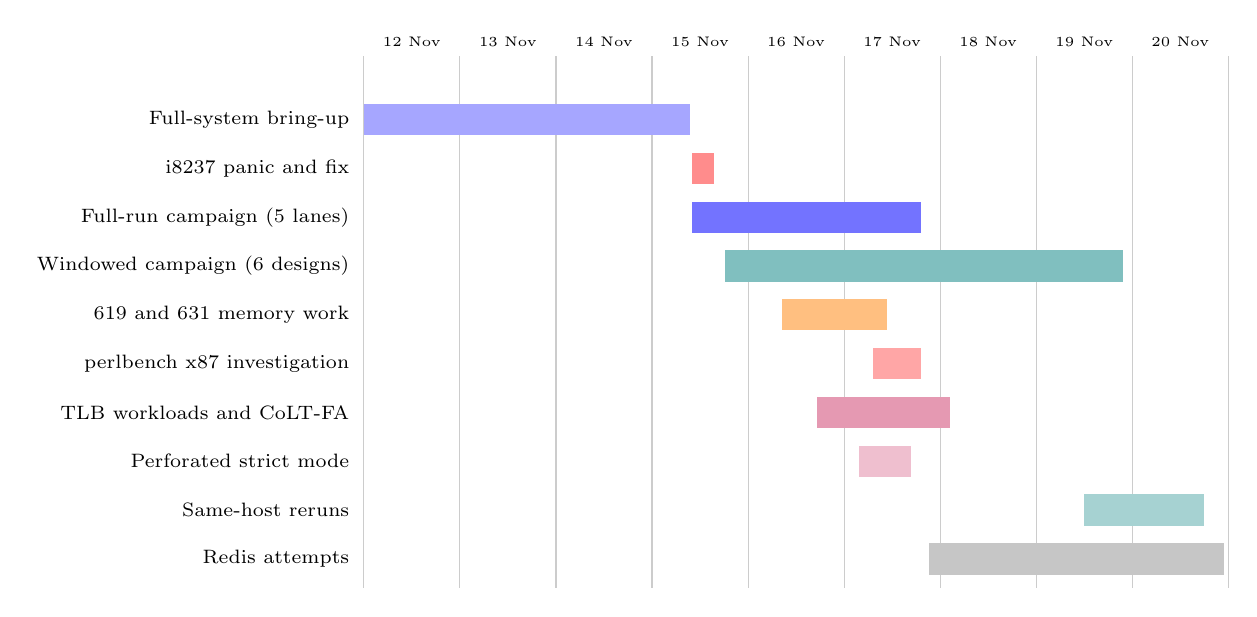
\begin{tikzpicture}[x=1.22cm, y=0.62cm, font=\scriptsize]
% day grid
\foreach \dd/\lab in {0/12 Nov,1/13 Nov,2/14 Nov,3/15 Nov,4/16 Nov,5/17 Nov,6/18 Nov,7/19 Nov,8/20 Nov} {
  \draw[gray!40] (\dd,0.3) -- (\dd,-10.6);
  \node[anchor=south, font=\tiny] at (\dd+0.5,0.3) {\lab};
}
\draw[gray!40] (9,0.3) -- (9,-10.6);
% rows: label, start, end, colour
\foreach \row/\lab/\st/\en/\col in {
 1/Full-system bring-up/0/3.4/blue!35,
 2/i8237 panic and fix/3.42/3.65/red!45,
 3/Full-run campaign (5 lanes)/3.42/5.8/blue!55,
 4/Windowed campaign (6 designs)/3.76/7.9/teal!50,
 5/619 and 631 memory work/4.35/5.45/orange!50,
 6/perlbench x87 investigation/5.3/5.8/red!35,
 7/TLB workloads and CoLT-FA/4.72/6.1/purple!40,
 8/Perforated strict mode/5.15/5.7/purple!25,
 9/Same-host reruns/7.5/8.75/teal!35,
 10/Redis attempts/5.88/8.95/gray!45} {
  \node[anchor=east] at (-0.05,-\row) {\lab};
  \fill[\col] (\st,-\row-0.32) rectangle (\en,-\row+0.32);
}
\end{tikzpicture}
\caption{Calendar of the second half of the project. Bars show when each activity was running, at the resolution of a few hours.}
\label{fig:chr_gantt}
\end{figure}

% -----------------------------------------------------------------------------
\section{The First Half: Building the Designs in SE Mode}
\label{sec:chr_phase1}
% -----------------------------------------------------------------------------

Part~\ref{part:mid} describes the first half in full. Here we only list its steps in order and what each step left behind for the second half (Table~\ref{tab:chr_phase1}).

\begin{table}[htbp]
\centering
\small
\caption{Steps of the first half, in order, with the open points each one left.}
\label{tab:chr_phase1}
\begin{tabularx}{\textwidth}{>{\raggedright\arraybackslash}p{3.2cm} X X}
\toprule
\textbf{Step} & \textbf{What was built and found} & \textbf{What it left open} \\
\midrule
Toolchain and baseline & \texttt{gem5} built for x86, static microbenchmarks, baseline TLB statistics. & Only SE mode was used. \\
Set-associative L2 & 128 sets, 4 ways, XOR-7 index, replacing the default L2 behaviour. & Index hash only tested on synthetic patterns. \\
Inclusion policies & Inclusive, NINE and Exclusive compared on microbenchmarks. & Invalidation of the L2 never exercised, since SE mode has no unmaps. \\
Prefetchers & Sequential and Naive Free Prefetching using the free PTEs in a cache line. & Fixed prefetch degree and direction. \\
CoLT-FA & Fully associative coalescing buffer, 52.19\% fewer L2 misses on its microbenchmark. & Coalescing read \texttt{gem5}'s emulated page table, which only exists in SE mode. \\
Perforated Pages & 2MB regions with a hole bitmap and a two-level filter; 4.16$\times$ speedup on clustered against dispersed holes. & The model kept a separate address for each 4KB page. \\
Hybrid L2 TLB & Combination of the mechanisms, 71.22\% fewer L2 misses. & Not continued in the second half. \\
Two discrepancies & CoLT looked useless next to huge pages; the coarse filter removed no walks in a functional model. & Both were explained at the mid-review (Section~7 of Part~\ref{part:mid}). \\
\bottomrule
\end{tabularx}
\end{table}

\noindent At the mid-review, the next steps listed in Section~9 of Part~\ref{part:mid} were new mechanisms from recent papers. After the review we changed direction. Since every number so far came from SE mode, we decided to first check that the designs are correct when a real kernel runs on top of them, and to measure them on real programs. The rest of this part follows that decision.

% -----------------------------------------------------------------------------
\section{Audit, Fixes and SE Verification}
\label{sec:chr_audit}
% -----------------------------------------------------------------------------

\subsection{What Was Done}
The audit, the fixes and the verification are described in detail in Part~\ref{part:post}. In time order they went as follows:
\begin{enumerate}
    \item Every design was read line by line against the \texttt{gem5} x86 TLB interface. The audit found that the L2 was not cleared when the kernel unmaps a page or switches address space, that L2 removal ignored the PCID, that checkpoints saved only the L1, and that Perforated hits used fixed permissions.
    \item Each design got its own fixed source files, so the original and the fixed version can be built and compared.
    \item A translation oracle and invariant checkers were added, and stress tests were written that unmap, remap and switch processes.
    \item Every design was run on the SE correctness matrix and on SPEC in SE mode.
\end{enumerate}

\subsection{What Went Wrong on the Way}
\begin{itemize}
    \item \textbf{The Inclusive checkpoint fix failed twice.} The checkpoint format was positional, so values written after the entry list were read back as part of the wrong section. This broke the first two fix attempts. The version that worked writes the L2 state in its own section.
    \item \textbf{Exclusive kept duplicate entries under SMT.} The checker found 391,950 violations in 1,368,154 checks before the fix and 0 after it.
    \item \textbf{Most fixed bugs cannot be reached in SE mode.} The unmap, CR3 and PCID paths are never used by SE programs, so passing in SE says little about them. This is what made a full-system campaign necessary.
    \item \textbf{SE mode redirects paths under \texttt{/tmp}.} A side check of 505.mcf\_r in SE mode printed \texttt{read error} and exited with code 255. A trace of system calls showed that SE mode had rewritten the input path \texttt{/tmp/.../inp.in} into \texttt{m5out/fs/tmp/.../inp.in}, where the file does not exist. Copying the file there did not help. The working solution, used for the SE SPEC runs, was to install and run SPEC from \texttt{/var/tmp} instead of \texttt{/tmp}. The same behaviour appeared again later in the perlbench investigation (Section~\ref{sec:chr_perl}).
\end{itemize}

% -----------------------------------------------------------------------------
\section{Bringing Up the Full-System Setup (12 to 15 November)}
\label{sec:chr_bringup}
% -----------------------------------------------------------------------------

\subsection{The Pieces}
A full-system run needs a kernel, a root disk image with Ubuntu 24.04, a second disk with the SPEC tree, a script that the guest runs after boot, and a configuration script for \texttt{gem5}. Figure~\ref{fig:chr_guestflow} shows how one run proceeds. The guest prints marker lines such as \texttt{SPEC\_START} and \texttt{SPEC\_RESULT} on its serial console, and the host side reads the console file to know what happened.

\begin{figure}[htbp]
\centering
\begin{tikzpicture}[
  node distance=0.3cm,
  st/.style={draw, rounded corners, fill=#1, minimum width=9.5cm, minimum height=0.62cm, align=left, font=\scriptsize, text width=9.3cm},
  st/.default=blue!6,
  side/.style={font=\tiny, text width=3.5cm, align=left},
  arr/.style={-{Stealth[length=1.8mm]}, thick}]
\node[st=gray!12] (s1) {\textbf{1.} \texttt{gem5} starts with the kernel, root image and SPEC disk (atomic CPU)};
\node[st, below=of s1] (s2) {\textbf{2.} Linux boots; systemd reaches the login prompt (about 2 hours under load)};
\node[st, below=of s2] (s3) {\textbf{3.} \texttt{after\_boot.sh} runs the generated guest script as user \texttt{gem5}};
\node[st, below=of s3] (s4) {\textbf{4.} Script re-runs itself with \texttt{sudo}, sets \texttt{ulimit -s unlimited}, mounts the SPEC disk};
\node[st, below=of s4] (s5) {\textbf{5.} For each benchmark: print \texttt{SPEC\_START}, run \texttt{runcpu --size=test}};
\node[st=green!10, below=of s5] (s6) {\textbf{6.} Check the runcpu log for \texttt{Success: 1x<benchmark>}; print \texttt{SPEC\_RESULT PASS} or \texttt{FAIL}};
\node[st=gray!12, below=of s6] (s7) {\textbf{7.} After the last benchmark: \texttt{sync}, print the completion marker, exit};
\foreach \a/\b in {s1/s2,s2/s3,s3/s4,s4/s5,s5/s6,s6/s7} \draw[arr] (\a) -- (\b);
\draw[arr] (s6.east) -- ++(0.5,0) |- (s5.east);
\node[side, right=0.9cm of s5] {loop over the benchmarks in the script};
\node[side, right=0.9cm of s2] {failure here: i8237 panic (Section~\ref{sec:chr_i8237})};
\node[side, right=0.9cm of s4] {failures here: sudo password, \texttt{shrc} path};
\node[side, right=0.9cm of s7] {wrong success string made every result FAIL};
\end{tikzpicture}
\caption{What happens inside one full-system run, with the places where the bring-up failed.}
\label{fig:chr_guestflow}
\end{figure}

Each lane of the full-run campaign was watched by a supervisor script running in its own terminal session. When a run failed, the supervisor wrote an incident file, marked the lane as blocked, and waited. A run was restarted by appending a line of the form \texttt{[ADMIN <time>] RESUME <lane>: <reason>} to a shared file. A shared status board read the heartbeat of each lane.

\subsection{Failures During Bring-Up, in Order}
Table~\ref{tab:chr_bringup} lists the problems met before the first complete launch. Each one stopped every lane, and each cost at least one boot of about 1.5 to 2 hours before it showed up.

\begin{table}[htbp]
\centering
\small
\caption{Problems found while bringing up the full-system runs.}
\label{tab:chr_bringup}
\begin{tabularx}{\textwidth}{>{\raggedright\arraybackslash}p{3.3cm} X X}
\toprule
\textbf{Symptom} & \textbf{Cause} & \textbf{Fix} \\
\midrule
Guest script stops at its first \texttt{sudo}. & The guest user is in the \texttt{sudo} group but \texttt{/etc/sudoers.d} was empty, so \texttt{sudo} asked for a password. & A drop-in sudoers file was written into each root image with \texttt{debugfs}, without booting it. \\
First two restart requests ignored. & The supervisor only accepted the bracketed \texttt{[ADMIN ...]} format. & Third attempt used the right format. \\
After the sudo fix, all five lanes blocked again in the morning. & The SPEC \texttt{shrc} script uses \texttt{pwd}, and it was sourced from the wrong directory. & Guest script generator changed to enter the SPEC directory first. \\
Every benchmark would have been marked FAIL. & The script searched for the wrong success string. \texttt{runcpu} prints \texttt{Success: 1x<benchmark>}. & Search string corrected. Since the pass cache is keyed on a hash of the generator, the edit also cleared old cached passes. \\
Four lanes kept running old guest scripts. & Generated scripts were not refreshed on the other hosts. & Scripts regenerated on every lane. \\
8 of 43 benchmarks fail natively (Table~\ref{tab:chr_native}). & Build problems in our SPEC configuration. & Configuration changes, after which all 43 passed natively on the Exclusive tree. \\
\bottomrule
\end{tabularx}
\end{table}

Before trusting any \texttt{gem5} result, the whole SPEC test set was run natively on a lab machine with the same binaries and configuration. 35 benchmarks passed and 8 failed (Table~\ref{tab:chr_native}).

\begin{table}[htbp]
\centering
\small
\caption{Benchmarks that failed natively with our first SPEC configuration.}
\label{tab:chr_native}
\begin{tabularx}{\textwidth}{>{\raggedright\arraybackslash}p{3.6cm} X X}
\toprule
\textbf{Benchmarks} & \textbf{What was seen} & \textbf{Fix} \\
\midrule
520.omnetpp\_r, 620.omnetpp\_s & Compile errors with the default C++ standard of the new compiler. & Built with \texttt{-std=gnu++14 -fpermissive}. \\
603.bwaves\_s, 621.wrf\_s, 627.cam4\_s, 628.pop2\_s, 649.fotonik3d\_s, 654.roms\_s & These Fortran OpenMP programs crashed. For bwaves, the debugger showed a call to address 0 inside the Fortran runtime. Raising the stack limit and the OpenMP stack size did not help. & In a static binary, references to the \texttt{pthread} functions are weak and were left unresolved. Linking with \texttt{-Wl,-u,<symbol>} for 17 symbols pulled them in. \\
627.cam4\_s & Needed a larger stack in addition to the above. & \texttt{ulimit -s unlimited} in the guest script. \\
\bottomrule
\end{tabularx}
\end{table}

\noindent On a second SPEC tree built later for the windowed campaign, 627.cam4\_s still failed its output check natively. Inside \texttt{gem5} it passed on every design where it finished. We report this as observed and did not investigate it further.

% -----------------------------------------------------------------------------
\section{First Launch and the i8237 Panic (15 November)}
\label{sec:chr_i8237}
% -----------------------------------------------------------------------------

All five lanes were restarted from scratch at about 10:05 on 15 November. On the Exclusive lane the atomic boot finished at about 11:29 and \texttt{SPEC\_START 500.perlbench\_r} appeared at 11:31. After that the console stayed silent.

\paragraph{A wrong first reading.} About 30 minutes later the \texttt{gem5} process was at 100\% CPU and the console had not changed. We read this as ``slow, not hung'' and decided not to act on silence alone. This was wrong. By 13:00 the process had disappeared on all five lanes, each with 43 rows of \texttt{FAIL missing-result-marker}. Those rows only meant that no benchmark had finished.

\paragraph{Narrowing down.} The host had not rebooted (uptime 3 days, load 0) and the supervisor was still alive, so the run had ended by itself. A first guess was a wall-clock timeout in the launch script, but a search of the script found none. The error file of the run held a backtrace inside the simulation loop, and its first lines gave the cause:
\begin{lstlisting}
src/dev/x86/i8237.cc:48: panic: Read from i8237 channel 0 current address unimplemented.
Program aborted at tick 14282334490878
\end{lstlisting}
The same panic was found on all five lanes. The i8237 is the legacy ISA DMA controller of the PC. The guest kernel reads one of its registers, and stock \texttt{gem5} stops with a panic for every register it does not model. This is a device-model gap and is unrelated to the TLB code.

\paragraph{Two patches.} The first patch changed the shared helpers for unimplemented registers to print one warning and return 0 on reads and ignore writes. Before relaunching, a search for every other \texttt{panic} and \texttt{fatal} in the PC device models found three more places in \texttt{i8237.cc} that the guest could reach: an illegal register read, enabling a channel, and requesting a DMA transfer. The second patch turned these into one-time warnings as well. The timer, CMOS and interrupt controller models also contain panics, but those are on register offsets outside the ranges the devices decode, so they were left unchanged. We did not prove that they are unreachable. Figure~\ref{fig:chr_i8237} shows the diagnosis.

\begin{figure}[htbp]
\centering
\begin{tikzpicture}[
  node distance=0.4cm and 0.6cm,
  q/.style={draw, diamond, aspect=2.6, fill=yellow!20, font=\scriptsize, align=center, inner sep=1pt, text width=2.6cm},
  b/.style={draw, rounded corners, fill=#1, font=\scriptsize, align=center, text width=3.3cm, minimum height=0.8cm},
  b/.default=blue!6,
  arr/.style={-{Stealth[length=1.8mm]}, thick}]
\node[b=gray!12] (a) {Console silent after \texttt{SPEC\_START}; \texttt{gem5} gone by 13:00};
\node[q, below=of a] (q1) {Host rebooted?};
\node[q, below=of q1] (q2) {Script timeout?};
\node[q, below=of q2] (q3) {Panic in error file?};
\node[b=green!10, below=of q3] (c) {\texttt{i8237.cc:48} panic on all five lanes};
\node[b=orange!15, below=of c] (p1) {Patch A: unimplemented reads return 0 with a warning};
\node[b=orange!15, below=of p1] (p2) {Scan all device panics; Patch B: three more i8237 sites};
\node[b=green!10, below=of p2] (ok) {Relaunch at about 15:15; main lanes then ran more than 16 hours with no panic};
\node[b=red!8, right=1.2cm of q1] (n1) {No: uptime 3 days};
\node[b=red!8, right=1.2cm of q2] (n2) {No: no time limit in the script};
\draw[arr] (a) -- (q1); \draw[arr] (q1) -- node[left, font=\tiny]{no} (q2); \draw[arr] (q2) -- node[left, font=\tiny]{no} (q3);
\draw[arr] (q3) -- node[left, font=\tiny]{yes} (c); \draw[arr] (c) -- (p1); \draw[arr] (p1) -- (p2); \draw[arr] (p2) -- (ok);
\draw[arr, dashed] (q1) -- (n1); \draw[arr, dashed] (q2) -- (n2);
\end{tikzpicture}
\caption{Diagnosis of the i8237 panic that stopped the first complete launch.}
\label{fig:chr_i8237}
\end{figure}

\paragraph{The cost.} The first relaunch was done right after Patch A, without first scanning for other reachable panics or running one test lane. When the scan found more cases, the five fresh runs were killed and restarted again at about 15:15, which cost another boot. A process note we adopted from this: check the error file for \texttt{panic} and \texttt{fatal} at every status check, and test a fix on one lane before relaunching all of them. Why the guest reads the DMA controller at all was never determined. The fix only makes the read harmless.

% -----------------------------------------------------------------------------
\section{Scaling the Full-Run Campaign (15 to 17 November)}
\label{sec:chr_scale}
% -----------------------------------------------------------------------------

\subsection{One Guest per Lane Was Too Slow}
The guest script runs the 43 benchmarks one after another. At about 17:00 on 15 November every lane was still on its first benchmark, and the deadline was close. Since the script had no way to run a subset, extra guests were added on idle cores. The 43 \texttt{SPEC\_START} blocks were split into $K$ slices, each slice became its own guest script, and each extra guest got its own copy of the SPEC disk. The main guest kept running the full list as the reference. Figure~\ref{fig:chr_extras} shows the layout.

\begin{figure}[htbp]
\centering
\begin{tikzpicture}[
  node distance=0.35cm and 0.35cm,
  h/.style={draw, rounded corners, fill=#1, font=\scriptsize, align=center, text width=2.4cm, minimum height=0.9cm},
  h/.default=blue!6,
  g/.style={draw, fill=green!10, font=\tiny, align=center, minimum width=0.9cm, minimum height=0.45cm},
  arr/.style={-{Stealth[length=1.6mm]}, thick}]
\node[h=gray!12] (gs) {Full guest script\\43 \texttt{SPEC\_START} blocks};
\node[h=orange!15, right=1.1cm of gs] (sp) {Split into $K$ slices\\(6 at first, later up to 16 per host)};
\node[h=blue!8, right=1.1cm of sp] (mk) {One SPEC disk copy\\per extra guest};
\draw[arr] (gs) -- (sp); \draw[arr] (sp) -- (mk);
\node[h=yellow!20, below=1.0cm of gs] (main) {Lane host\\main guest + extras};
\node[h=yellow!20, right=0.6cm of main] (x1) {Extra host 1\\several guests};
\node[h=yellow!20, right=0.6cm of x1] (x2) {Extra host 2\\several guests};
\node[right=0.3cm of x2, font=\scriptsize] (dots) {\dots};
\node[h=yellow!20, right=0.3cm of dots] (xn) {Extra host $n$\\up to 64 hosts};
\draw[arr] (mk.south) -- ++(0,-0.45) -| (x1.north);
\draw[arr] (mk.south) -- ++(0,-0.45) -| (x2.north);
\draw[arr] (mk.south) -- ++(0,-0.45) -| (xn.north);
\draw[arr] (mk.south) -- ++(0,-0.45) -| (main.north);
\node[h=gray!12, below=0.8cm of x2, text width=8cm] (mon) {Each host writes a status file into the shared home; one board script reads all of them (\texttt{fullview})};
\draw[arr, dashed] (main.south) -- (mon); \draw[arr, dashed] (x1.south) -- (mon); \draw[arr, dashed] (xn.south) -- (mon);
\end{tikzpicture}
\caption{How the full-run campaign was spread over many machines by splitting the guest script.}
\label{fig:chr_extras}
\end{figure}

\noindent The number of extra guests per host was first fixed at 6 and later chosen from the free disk space, since each SPEC disk copy takes about 15 to 17GB. By the morning of 16 November 30 hosts were reporting, and by 17 November 64 hosts, with up to 87 guests per lane and more than 1,000 CPU-hours spent per lane.

\subsection{Monitoring Problems}
A first board script logged into each lane host over SSH. On the machine where it was run, the \texttt{ssh} program itself crashed with a segmentation fault, so every lane showed \texttt{SSH\_FAILED}. The board was rebuilt so that each host writes its own report into the shared home directory and the board only reads those files. It also showed old incident files as new, because its default cut-off time was too early. The monitor still could not tell a slow run from a hung one after \texttt{SPEC\_START}, which is the same blind spot that caused the wrong reading on 15 November.

\subsection{Results of the Full-Run Campaign}
Table~\ref{tab:chr_fullrun} gives the last complete status of this campaign that was recorded, at 15:42 on 17 November, together with the 12 GiB runs of Section~\ref{sec:chr_mem}. These runs used the timing CPU for the whole benchmark, so they are an independent check of the five designs from the windowed campaign.

\begin{table}[htbp]
\centering
\small
\caption{Full-run campaign, status recorded at 15:42 on 17 November (SPEC test inputs, out of 43).}
\label{tab:chr_fullrun}
\begin{tabularx}{\textwidth}{l c X}
\toprule
\textbf{Design} & \textbf{PASS} & \textbf{FAIL at that time} \\
\midrule
Inclusive & 35 & 600.perlbench\_s, 619.lbm\_s, 631.deepsjeng\_s (3 GiB) \\
Exclusive & 35 & 500.perlbench\_r, 600.perlbench\_s, 631.deepsjeng\_s (3 GiB) \\
NINE & 35 & 500.perlbench\_r, 600.perlbench\_s, 619.lbm\_s, 631.deepsjeng\_s (3 GiB) \\
Agile / NaiveFP & 35 & 500.perlbench\_r, 619.lbm\_s, 631.deepsjeng\_s (3 GiB) \\
Perforated Pages & 35 & 500.perlbench\_r, 600.perlbench\_s, 631.deepsjeng\_s (3 GiB) \\
\midrule
\multicolumn{3}{l}{631.deepsjeng\_s on the 12 GiB board: PASS on all five designs.} \\
\bottomrule
\end{tabularx}
\end{table}

\noindent The remaining benchmarks were still running at that time. The failures are the same kinds as in the windowed campaign: perlbench, and the two benchmarks that need more memory than the guest has. The next three sections describe how each of these was investigated.

% -----------------------------------------------------------------------------
\section{The Windowed Campaign (15 to 19 November)}
\label{sec:chr_window}
% -----------------------------------------------------------------------------

\subsection{Why a Second Campaign}
On the evening of 15 November it was clear that running whole benchmarks on the timing CPU would not finish all 43 benchmarks on all designs in time, and that cycle and IPC numbers were needed for the performance study. A second campaign was started with three differences: one \texttt{gem5} process per benchmark instead of one guest per lane, the atomic CPU for everything except a measurement window, and CoLT-FA as a sixth design from 16 November. Figure~\ref{fig:chr_window} shows the life of one windowed run.

\begin{figure}[htbp]
\centering
\begin{tikzpicture}[
  node distance=0.5cm and 0.55cm,
  s/.style={draw, rounded corners, fill=#1, font=\scriptsize, align=center, text width=2.1cm, minimum height=1.0cm},
  s/.default=blue!6,
  arr/.style={-{Stealth[length=1.8mm]}, thick}]
\node[s=gray!12] (b) {Boot\\atomic CPU};
\node[s, right=of b] (r) {\texttt{runcpu} setup\\atomic};
\node[s=yellow!20, right=of r] (w) {Warm-up\\50M instr.\\atomic};
\node[s=green!12, right=of w] (t) {Window\\200M instr.\\timing CPU};
\node[s=orange!15, right=of t] (d) {Dump\\statistics};
\node[s, below=0.9cm of d] (a2) {Back to atomic\\to the end};
\node[s=gray!12, left=of a2] (res) {Output check\\\texttt{SPEC\_RESULT}};
\draw[arr] (b) -- (r); \draw[arr] (r) -- node[above, font=\tiny]{exe starts} (w); \draw[arr] (w) -- (t); \draw[arr] (t) -- (d);
\draw[arr] (d) -- (a2); \draw[arr] (a2) -- (res);
\node[font=\tiny, text width=4.2cm, align=left, left=0.4cm of res] {Hypercalls 11 and 12 from the SPEC \texttt{submit} wrapper mark where the benchmark executable starts and ends};
\end{tikzpicture}
\caption{The phases of one run in the windowed campaign.}
\label{fig:chr_window}
\end{figure}

\subsection{Events in Order}
\begin{itemize}
    \item \textbf{15 November, 18:20.} The first shards were launched on the same lane hosts as the full-run campaign. At about 21:15 the shared load had slowed the full-run boots from about 100 minutes to more than 3 hours, and we were asked to move. About 70 idle lab machines were found that accepted our login. Earlier attempts had failed only because SSH asked to confirm unknown host keys, which batch mode cannot answer. The runs were moved to 10 machines, two per design, with 215 runs in all.
    \item \textbf{16 November, 03:50. The window handler bug.} Six runs had ended right at the end of their window, with no statistics and no SPEC result. The configuration had registered the instruction-count handler as a one-element list. In \texttt{gem5} 25.1 a list is treated as a queue of handlers, each used once, so the second instruction-count event fell through to the default handler, which ends the simulation. Every benchmark would have hit this. The handler was changed to a single function, which runs on every event. At the same time the warm-up was lowered from 500M to 50M instructions, because some test inputs are shorter than 500M. All 215 runs were restarted at 03:47.
    \item \textbf{16 November, 15:25.} 130 windows had been dumped. Three runs had crashed when switching from the timing CPU back to the atomic CPU, all on 619.lbm\_s (Section~\ref{sec:chr_lbm}). There was still no SPEC result anywhere.
    \item \textbf{16 November, 16:46. First result.} Exclusive 623.xalancbmk\_s passed. Its executable had only about 0.4G instructions but the run took 8 to 9 hours after \texttt{SPEC\_START}, which showed that the setup and output checking of \texttt{runcpu} under the atomic CPU take about 8 hours. With a measured atomic speed of about 0.9 million instructions per second, the finish time of a benchmark was estimated as \texttt{SPEC\_START} + 8 hours + 0.31 hours per billion native instructions. This model gave the ETAs for the rest of the campaign. The two x264 benchmarks, at about 1 trillion instructions each, would need about 13 days and were not completed.
    \item \textbf{16 November, 17:30.} The windows showed that SPEC test inputs barely use the TLB (Section~\ref{sec:fs_spec}). This started the TLB-intensive workload sets of Section~\ref{sec:chr_workloads}.
    \item \textbf{17 November.} Several machines went offline or were rebooted, and their runs were moved. The 9 longest benchmarks were also rerun on lightly loaded machines, about a day ahead of the packed copies. perlbench failed on every design that reached it (Section~\ref{sec:chr_perl}).
    \item \textbf{19 November, 23:30.} The final matrix was 37 PASS on four designs, 36 PASS on Agile and CoLT-FA with 627.cam4\_s still running, and the same three failures everywhere.
\end{itemize}

\subsection{Other Problems of This Campaign}
\begin{itemize}
    \item \textbf{Home quota.} The NFS home directory has a quota of about 10GB, while one design's inputs are about 20GB. Inputs were copied directly between lab machines over SSH instead.
    \item \textbf{No KVM.} \texttt{/dev/kvm} on the lab machines is granted only to the user logged in at the console, so every boot used the atomic CPU.
    \item \textbf{The laptop slept.} The result mirror ran on a laptop. Three times the laptop went to sleep and the copy loop died, so it was made to keep connections alive and restarted. No results were lost because every result also stays on its lab machine until copied.
    \item \textbf{Load.} One \texttt{gem5} ran at 2.23 million instructions per second on an idle machine and at 0.58 on a machine with about 30 \texttt{gem5} processes. A full machine still did about 7 times more work in total.
\end{itemize}

% -----------------------------------------------------------------------------
\section{619.lbm\_s: A Page Walker Write in the Cache Hierarchy}
\label{sec:chr_lbm}
% -----------------------------------------------------------------------------

619.lbm\_s crashed \texttt{gem5} in both campaigns, in different ways. Figure~\ref{fig:chr_lbm} shows the chain of failures and changes.

\begin{figure}[htbp]
\centering
\begin{tikzpicture}[
  node distance=0.45cm and 0.5cm,
  c/.style={draw, rounded corners, fill=red!8, font=\scriptsize, align=center, text width=3.6cm, minimum height=0.9cm},
  f/.style={draw, rounded corners, fill=orange!15, font=\scriptsize, align=center, text width=3.6cm, minimum height=0.9cm},
  o/.style={draw, rounded corners, fill=green!10, font=\scriptsize, align=center, text width=3.6cm, minimum height=0.9cm},
  arr/.style={-{Stealth[length=1.8mm]}, thick}]
\node[c] (c1) {Crash 1: failure in \texttt{coherent\_xbar.cc:159}};
\node[f, below=of c1] (f1) {Change 1: walker writes the page table entry back with its own write request};
\node[c, below=of f1] (c2) {Crash 2: \texttt{cache.cc:1225} ``passing a Modified line through WriteReq, but keeping the block''};
\node[f, below=of c2] (f2) {Change 2: the PTE write is done functionally, taking no simulated time};
\node[c, below=of f2] (c3) {3 GiB guest: kernel kills lbm for lack of memory (2.7GB resident)};
\node[o, below=of c3] (o1) {SE mode with 8 GiB: PASS on all six designs};
\node[c, right=1.4cm of c1] (w1) {Windowed campaign: assertion in \texttt{Cache::handleSnoop} when switching from timing back to atomic};
\node[o, below=of w1] (w2) {Window statistics were already dumped and are kept};
\node[o, below=of w2] (w3) {Native check: lbm\_s needs 3.2GB, above the 3 GiB guest};
\draw[arr] (c1) -- (f1); \draw[arr] (f1) -- (c2); \draw[arr] (c2) -- (f2); \draw[arr] (f2) -- (c3); \draw[arr] (c3) -- (o1);
\draw[arr] (w1) -- (w2); \draw[arr] (w2) -- (w3); \draw[arr] (w3.south) |- (o1.east);
\node[above=0.15cm of c1, font=\scriptsize\bfseries] {Full-run campaign};
\node[above=0.15cm of w1, font=\scriptsize\bfseries] {Windowed campaign};
\end{tikzpicture}
\caption{The sequence of failures and changes for 619.lbm\_s.}
\label{fig:chr_lbm}
\end{figure}

\paragraph{Full-run campaign.} The first crash was a failure in the coherent crossbar (\texttt{coherent\_xbar.cc:159}). A first change to how the walker writes a page table entry back to memory moved the crash to a different place, \texttt{cache.cc:1225}:
\begin{lstlisting}
panic condition !invalidate && !pkt->hasSharers() occurred:
board.cache_hierarchy.l1d-cache-0 is passing a Modified line through WriteReq
[14a3c5b8:14a3c5bf], but keeping the block
\end{lstlisting}
The backtrace ended in the walker's retry of a request (\texttt{Walker::WalkerPort::recvReqRetry}). Reading the cache code showed why. When a snoop finds a dirty line, the cache only gives up the line if the incoming packet is an invalidating request, and \texttt{invalidate} is taken from \texttt{pkt->isInvalidate()}. A plain \texttt{WriteReq}, which the walker sends, does not carry that attribute, so the cache is asked to pass on a Modified line while also keeping it. The cache code itself has a comment saying that this case is not handled.

A control run with unmodified \texttt{gem5} was set up to tell whether this is a stock bug. It died early on the unpatched i8237 panic of Section~\ref{sec:chr_i8237}, so the question stayed open. The second change made the walker's page table write functional, so it updates memory directly and takes no simulated time. \textbf{This is a deviation from stock \texttt{gem5}} and it only affects one write per first-touch page walk. Building it first failed on four lanes with a missing \texttt{GLIBCXX} symbol version, because the new binary needs the newer C++ library that the lab machines only have in a separate directory. Setting \texttt{LD\_LIBRARY\_PATH} fixed the build and the launch.

With the second change, the 3 GiB runs no longer crashed. \texttt{gem5} exited normally, but the benchmark result was \texttt{FAIL}: the guest console showed that the kernel had killed 619.lbm\_s for lack of memory, with about 2.7GB resident. Runs of 619.lbm\_s on the 12 GiB board (Section~\ref{sec:chr_mem}) were started on 17 November, but no result was recorded before the end of the campaign.

\paragraph{Windowed campaign.} Here 619.lbm\_s crashed on every design where it was reached, always just after its window, when the run switched from the timing CPU back to the atomic CPU. The assertion was \texttt{Packet::setCacheResponding} in \texttt{Cache::handleSnoop}, reached from an atomic access by the walker. This is the same family of problem: a walker access meeting a dirty line during the CPU switch. The window statistics had already been dumped. A native measurement then showed that 619.lbm\_s needs 3.2GB, so it could not pass in a 3 GiB guest anyway. Both campaigns therefore used SE mode with 8 GiB for its pass/fail result (Section~\ref{sec:fs_spec}).

% -----------------------------------------------------------------------------
\section{631.deepsjeng\_s and a 12 GiB Board}
\label{sec:chr_mem}
% -----------------------------------------------------------------------------

631.deepsjeng\_s needs about 6.7 to 6.9GB of memory. In both campaigns it failed in the 3 GiB guest. In the windowed campaign its executable ended almost at once, which first showed up as a window that was too short. In the full-run campaign it ended with \texttt{FAIL rc=0}, and some copies were killed by the kernel for lack of memory.

\paragraph{Why 3 GiB.} On a PC, the address range just below 4GB is used by devices, so memory above 3GB has to be placed above 4GB and described to the kernel in the E820 memory map. Figure~\ref{fig:chr_e820} shows the layout. The board used by both campaigns only described memory below the device range.

\begin{figure}[htbp]
\centering
\begin{tikzpicture}[x=1cm, y=0.5cm, font=\scriptsize]
\draw[fill=green!15] (0,0) rectangle (6,1); \node at (3,0.5) {RAM, 0 to 3GB (E820 entry, always present)};
\draw[fill=gray!25] (6,0) rectangle (8,1); \node at (7,0.5) {devices, 3 to 4GB};
\draw[fill=blue!15] (8,0) rectangle (14,1); \node at (11,0.5) {RAM above 4GB (added E820 entry)};
\foreach \x/\l in {0/0,6/3GB,8/4GB,14/13GB} \node[below] at (\x,0) {\l};
\draw[-{Stealth}] (11,2.6) -- (11,1.1);
\node[align=center, text width=6cm] at (11,3.6) {first attempt: entry created inline, \texttt{gem5} refused it as an ``orphan node''};
\draw[-{Stealth}] (3,2.6) -- (3,1.1);
\node[align=center, text width=5cm] at (3,3.6) {3 GiB board: guest sees only this part};
\end{tikzpicture}
\caption{Guest physical memory on the 12 GiB board. The extra memory has to be placed above the device range and described in the E820 table.}
\label{fig:chr_e820}
\end{figure}

\paragraph{The 12 GiB board.} A separate configuration script set the memory size to 12 GiB and appended an E820 entry starting at 4GB for the rest. Its first launch failed during configuration with \texttt{RuntimeError: Attempt to instantiate orphan node <orphan X86E820Entry>}. In \texttt{gem5}, every simulation object must belong to a parent object, and the new entry had been created inside a list expression without one. Storing the entry as an attribute of the workload before adding it to the table fixed the error, and the guest kernel then reported the extra memory range. The same restart also removed a launch script that had been started twice on four hosts, so two copies had been working on the same files.

\paragraph{Result.} On the 12 GiB board, 631.deepsjeng\_s passed in full-system mode on all five designs of the full-run campaign. Separately, it passed in SE mode with 8 GiB on all six designs, with output identical to the native run. A native memory probe at the same time also showed that 627.cam4\_s did not crash because of the memory limit, and that it completed when run with one OpenMP thread and a 1GB OpenMP stack.

% -----------------------------------------------------------------------------
\section{perlbench: Finding an x87 Emulation Bug}
\label{sec:chr_perl}
% -----------------------------------------------------------------------------

This was the longest investigation of the project. Both 500.perlbench\_r and 600.perlbench\_s failed on every design in both campaigns, so the cause was not any one TLB design. Figure~\ref{fig:chr_perl} shows the order in which possible causes were removed.

\begin{figure}[htbp]
\centering
\begin{tikzpicture}[
  node distance=0.32cm and 0.5cm,
  b/.style={draw, rounded corners, fill=#1, font=\scriptsize, align=left, text width=6.6cm, minimum height=0.6cm},
  b/.default=blue!6,
  x/.style={draw, rounded corners, fill=red!8, font=\scriptsize, align=left, text width=4.4cm, minimum height=0.6cm},
  arr/.style={-{Stealth[length=1.6mm]}, thick}]
\node[b=gray!12] (s0) {FAIL on every design; \texttt{op/sprintf2.t} tests 1409 and 1444 print \texttt{-0x0p+0} for \texttt{\%a} of 0};
\node[b, below=of s0] (s1) {Same binary passes natively};
\node[b, below=of s1] (s2) {Passes natively with the exact guest wrapper; fails in \texttt{gem5} without it};
\node[b, below=of s2] (s3) {Reproduced in SE mode in seconds with a 5-line perl script};
\node[b=orange!15, below=of s3] (s4) {Warning: \texttt{fcomip} unimplemented. Fix 1: implement it};
\node[b, below=of s4] (s5) {Single values now right, but \texttt{(0,1)} prints \texttt{0x1p+1} instead of \texttt{0x1p+0}};
\node[b, below=of s5] (s6) {Small C test programs: earlier x87 instructions leave state behind};
\node[b, below=of s6] (s7) {\texttt{fld1} loads 0 and \texttt{flds 2.0} loads 0 in \texttt{gem5}};
\node[b=orange!15, below=of s7] (s8) {Fix 2: x87 \texttt{movfp} micro-ops copy all 64 bits (\texttt{dataSize=8})};
\node[b=green!10, below=of s8] (s9) {30 of 30 checks match native, including perl \texttt{\%a} cases};
\foreach \a/\b in {s0/s1,s1/s2,s2/s3,s3/s4,s4/s5,s5/s6,s6/s7,s7/s8,s8/s9} \draw[arr] (\a) -- (\b);
\node[x, right=of s1] (r1) {Not the binary or the SPEC setup};
\node[x, right=of s2] (r2) {Not the submit wrapper or the window hypercalls};
\node[x, right=of s3] (r3) {Guessed \texttt{movmskpd}: ruled out};
\node[x, right=of s6] (r6) {Ruled out: \texttt{fstp} flags, missing \texttt{fstl}, \texttt{fxch}, 80-bit conversion, \texttt{fstpt}};
\foreach \a/\b in {s1/r1,s2/r2,s3/r3,s6/r6} \draw[arr, dashed] (\a) -- (\b);
\end{tikzpicture}
\caption{Order in which possible causes of the perlbench failure were removed.}
\label{fig:chr_perl}
\end{figure}

\subsection{From the Failure to a Small Reproduction}
The perl test log, read from inside the guest's SPEC disk image, showed that 316 of 317 checks in \texttt{op/sprintf2.t} passed. The two failures were both \texttt{\%a} formatting of zero, printed as \texttt{-0x0p+0} instead of \texttt{0x0p+0}. Natively the same binary passed. In the windowed campaign we also confirmed that both perlbench benchmarks pass natively with the exact guest submit wrapper (with the \texttt{gem5} hypercall program replaced by \texttt{/bin/true}), and a run inside \texttt{gem5} with no wrapper at all still failed. So the cause was in how \texttt{gem5} executes the program.

A first guess was the \texttt{movmskpd} instruction, which C libraries use to read the sign of a double. \texttt{gem5} implements it, and reading its micro-op showed that it would return the right sign for $+0.0$, so the guess was dropped. A first attempt to run perl in SE mode failed because perl could not open its script under \texttt{/tmp}, which is the path redirection of Section~\ref{sec:chr_audit}. With the script in the home directory, the bug appeared in seconds:
\begin{lstlisting}
script:  printf("%a %a %.13a\n", 0, 1, 0);
native:  0x0p+0 0x1p+0 0x0.0000000000000p+0
gem5:    -0x0p+0 -0x1p+1 -0x0.0000000000000p+0
warn: instruction 'fcomip' unimplemented
\end{lstlisting}

\subsection{First Cause: \texttt{fcomip} Was a Stub}
\texttt{fcomip} compares two x87 registers, sets the flags and pops the stack. In \texttt{gem5} it was decoded but did nothing. In the perl binary it comes right before the sign test, so the flags it should set were stale. Implementing \texttt{fcomip} fixed single values, but printing several values in one call was still wrong: \texttt{(0,1)} gave \texttt{0x0p+0 0x1p+1} instead of \texttt{0x0p+0 0x1p+0}.

\subsection{Second Cause: 32-bit Register Moves}
The multi-value case took most of the time. The perl code involved is a short x87 sequence:
\begin{lstlisting}
fldz; fld %st(0); fldt 0x30(%rsp); fmul %st(2),%st; fucomip %st(1),%st; fstp %st(0); jp; jz
\end{lstlisting}
A series of small C programs, each with inline assembly and each changing one thing, was run natively and in \texttt{gem5}. Table~\ref{tab:chr_x87tests} lists them. Several hypotheses were made and dropped on the way: that \texttt{fstp} clobbers the zero flag, that a missing \texttt{fstl} is the cause, that \texttt{fxch} is wrong, that conversion to and from 80-bit values is wrong, and that \texttt{fstpt} leaves bad state. Two of our own readings were also wrong for a while: one test that seemed to pass was not a real test, because \texttt{1.0L} itself read as zero in \texttt{gem5}, and ``process state is ruled out'' was withdrawn when a failing test was found to run after other x87 code in the same process.

\begin{table}[htbp]
\centering
\small
\caption{The x87 test programs used to find the second cause.}
\label{tab:chr_x87tests}
\begin{tabularx}{\textwidth}{l X X}
\toprule
\textbf{Test} & \textbf{What it varied} & \textbf{What it showed} \\
\midrule
W1 to W6 & Variants of the perl sequence in a fresh process & All matched native, so the sequence alone does not fail \\
U1 to U3 & 80-bit round trip and flags & U1 and U3 failed in \texttt{gem5} on the current build \\
X1 to X6 & One change at a time from U3 & All matched in a fresh process \\
Y1 to Y5 & Different x87 code run before U3 & A balanced \texttt{fldl; fstpt} before it made it fail \\
Z1 to Z4 & Printed the actual values & A plain \texttt{fldl; fstpl} was enough; a stale 1.0 sat where \texttt{fldz} should give 0 \\
D0 to D3 & 4 kinds of earlier code $\times$ 3 probes & Register-only push and pop is clean; a memory load with \texttt{fldl} leaves bad state \\
R0 to R9 & Which earlier load or store & Only cases with \texttt{fldl} fail; \texttt{fld1}, \texttt{flds}, \texttt{fstl} pass \\
S0 to S4 & Constants and single loads & \texttt{fld1} loads 0 and \texttt{flds 2.0} loads 0 in \texttt{gem5} \\
\bottomrule
\end{tabularx}
\end{table}

The S tests pointed to the micro-op that moves a value into an x87 register. Most x87 instructions in \texttt{gem5} are built from a load or constant into a temporary register, followed by \texttt{movfp} into the stack slot. \texttt{movfp} has a 4-byte mode, used by SIMD instructions such as \texttt{movss}, that copies only the low 32 bits and keeps the old high 32 bits of the destination. The x87 instructions did not set a data size, so their \texttt{movfp} ran in the 4-byte mode. A double has its sign, exponent and top of the fraction in the high 32 bits, so the destination kept those bits from whatever value was in that slot before (Figure~\ref{fig:chr_movfp}). This is why earlier x87 code changed later results, and why constants such as 1.0 and 2.0, whose low 32 bits are zero, loaded as zero or as an old value.

\begin{figure}[htbp]
\centering
\begin{tikzpicture}[x=0.11cm, y=0.55cm, font=\scriptsize]
\node[anchor=east] at (-2,2.5) {old slot (1.0)};
\draw[fill=red!15] (0,2) rectangle (32,3); \node at (16,2.5) {\texttt{3FF00000}};
\draw[fill=gray!10] (32,2) rectangle (64,3); \node at (48,2.5) {\texttt{00000000}};
\node[anchor=east] at (-2,0.5) {new value (0.0)};
\draw[fill=gray!10] (0,0) rectangle (32,1); \node at (16,0.5) {\texttt{00000000}};
\draw[fill=green!15] (32,0) rectangle (64,1); \node at (48,0.5) {\texttt{00000000}};
\node[anchor=east] at (-2,-1.5) {result, 4-byte move};
\draw[fill=red!15] (0,-2) rectangle (32,-1); \node at (16,-1.5) {\texttt{3FF00000}};
\draw[fill=green!15] (32,-2) rectangle (64,-1); \node at (48,-1.5) {\texttt{00000000}};
\node[anchor=west, text width=4.2cm] at (67,-1.5) {= 1.0, not 0.0: the high half was never written};
\node[above] at (16,3) {high 32 bits}; \node[above] at (48,3) {low 32 bits};
\draw[-{Stealth}, thick] (48,0) -- (48,-0.95);
\end{tikzpicture}
\caption{Effect of the 4-byte \texttt{movfp} on an x87 register: loading 0.0 into a slot that held 1.0 leaves 1.0.}
\label{fig:chr_movfp}
\end{figure}

\paragraph{The fix.} \texttt{dataSize=8} was added to the 22 \texttt{movfp} lines in the x87 instruction definitions. The 12 SIMD files that also use \texttt{movfp} were left alone, since \texttt{movss} needs the 32-bit behaviour. All five design builds were patched and rebuilt. On the Exclusive build, 30 of 30 checks matched native: the S, Q, R, Y and Z tests and three perl \texttt{\%a} scripts, including the \texttt{(0,1,0)} case.

\paragraph{Full-system reruns.} Relaunching 500.perlbench\_r and 600.perlbench\_s on the fixed builds took several tries. A text substitution in the launch script did not match the line it was meant to change, so two lanes copied into an old directory. One lane had its work files under a different directory name. All lanes then exited at once because the new binary needs \texttt{LD\_LIBRARY\_PATH} for the newer C++ library, which the launch command did not set. The ten guests were finally running at about 18:50 on 17 November with no panics, but no result from them was recorded before the end of the campaign. The fixed builds also used the original page walker, without the functional write of Section~\ref{sec:chr_lbm}.

\paragraph{What remains open.} Whether \texttt{1.0L} reading as zero is a third, separate bug was not checked. Whether other unimplemented x87 instructions, such as \texttt{fxam}, matter was not checked. All other SPEC results were produced by builds without these fixes. Benchmarks that passed are not affected in their pass/fail outcome, but an x87-heavy program could have taken a different path.

% -----------------------------------------------------------------------------
\section{TLB-Intensive Workloads and CoLT-FA (16 to 18 November)}
\label{sec:chr_workloads}
% -----------------------------------------------------------------------------

\subsection{Why New Workloads}
On 16 November the first windows showed that SPEC test inputs give almost no TLB pressure: the highest value on the Inclusive design was 1.145 page walks per 1000 instructions. The designs would therefore look the same on SPEC test inputs. Three sets of TLB-intensive runs were started the same evening.
\begin{enumerate}
    \item \textbf{Microbenchmarks}, including a GUPS random update kernel and pointer chasing over 256MB.
    \item \textbf{SPEC reference inputs} for nine memory-heavy benchmarks, with a 3G-instruction warm-up and a 200M-instruction window.
    \item \textbf{Well-known benchmarks}, since we preferred standard suites over our own programs: GAPBS, XSBench, STREAM and memcached. The lab machines cannot reach GitHub, so the sources were downloaded on a laptop, copied over, and built as static binaries. GAPBS graphs were generated in advance, because generating them took about 95\% of the instructions of a run.
\end{enumerate}

\subsection{CoLT-FA Becomes the Sixth Design}
The instructor had asked us to focus on CoLT. At about 18:30 on 16 November CoLT-FA was added to the full-system campaign. The mid-review version could not work under a real kernel, since it read \texttt{gem5}'s emulated page table. It was rebuilt on the fixed NINE design so that the hardware page walker builds coalesced runs from the eight page table entries in the cache line it has just read (Section~\ref{sec:colt_fs}). A switch, \texttt{COLT\_ENABLE=0}, turns the buffer off, so the same binary also runs plain NINE. This later turned out to be important for fair comparisons. CoLT-FA was first verified in SE mode with the oracle (36 of 36 runs) and then launched on all sets.

\subsection{The Instructor's Suggestion}
On 17 November the instructor suggested running a graph benchmark (GAPBS) and a key-value store (Redis or memcached). GAPBS bfs, pr and cc and memcached were already running. The set was extended with GAPBS bc, sssp and tc, and with Redis 7.2.5 built statically.

\subsection{Two Results That Needed a Second Look}
\paragraph{Perforated Pages looked too good.} On 17 November Perforated Pages showed close to zero walks on almost every workload, for example 0.24 against 54.76 for NINE on pr. Reading the model showed that each L2 entry stored a separate physical address for each of the 512 pages of its 2MB region and never checked physical contiguity, which gives about 512 times the reach of a real design. A strict mode was written the same day and run on the same workloads. Under the strict rule Perforated Pages had more walks than NINE on most workloads (Section~\ref{sec:perf_strict}). This also changes how the Perforated results of Part~\ref{part:mid} should be read.

\paragraph{CoLT-FA looked worse with huge pages on.} On 18 November a comparison with huge pages on gave NINE 2.16 and CoLT-FA 4.31 walks per 1000 instructions for bc. The CoLT-FA run had millions of buffer hits, which meant its guest had used many more 4KB pages than the NINE run. The two runs came from different machines, and each machine had built its own disk image. Repeating a run on the same machine gave exactly the same statistics, while the same NINE configuration gave 2.16 on one machine and 6.04 on another. We concluded that with huge pages on, results depend on the machine, and adopted the rule that such results are only compared between runs on the same machine. NINE and CoLT-FA were rerun in pairs on single machines on 20 November (Table~\ref{tab:colt_thpon}). With 4KB pages the results were stable across machines, so those comparisons stand. Figure~\ref{fig:chr_samehost} illustrates the rule.

\begin{figure}[htbp]
\centering
\begin{tikzpicture}[
  node distance=0.4cm and 0.6cm,
  m/.style={draw, rounded corners, fill=#1, font=\scriptsize, align=center, text width=3.2cm, minimum height=1.0cm},
  arr/.style={-{Stealth[length=1.8mm]}, thick}]
\node[m=blue!8] (a) {\textbf{Machine A}\\own disk image A\\huge page layout A};
\node[m=blue!8, right=2.4cm of a] (b) {\textbf{Machine B}\\own disk image B\\huge page layout B};
\node[m=green!10, below=of a] (a1) {NINE and CoLT-FA\\both on A: compared};
\node[m=green!10, below=of b] (b1) {NINE and CoLT-FA\\both on B: compared};
\coordinate (mid) at ($(a)!0.5!(b)$);
\node[m=red!8, below=2.9cm of mid] (x) {NINE on A against\\CoLT-FA on B: not compared};
\draw[arr] (a) -- (a1); \draw[arr] (b) -- (b1);
\draw[arr, dashed] (a) -- (x); \draw[arr, dashed] (b) -- (x);
\end{tikzpicture}
\caption{The same-machine rule for results with huge pages on.}
\label{fig:chr_samehost}
\end{figure}

\subsection{Redis}
Redis was prepared as the second key-value store. In the first runs every configuration stopped making progress inside the guest before the measured phase, and the runs were stopped after about two days. A first guess was that the guest was waiting for random numbers, but a diagnostic run showed that the random number generator was ready 2.6 seconds into the boot and that the server answered a ping. The driver was then changed to wait for the server's ready message before starting the load, to use fewer keys, and to print a progress line at every step. The second attempt also stopped, right after starting the server, and printed nothing for six hours. With the submission deadline close, Redis was left out, and memcached covers the key-value store case.

% -----------------------------------------------------------------------------
\section{Final Measurements, Report and Artifact (19 to 20 November)}
\label{sec:chr_final}
% -----------------------------------------------------------------------------

\begin{itemize}
    \item The windowed campaign finished apart from 627.cam4\_s on two designs and the two x264 benchmarks. Result files from all machines were gathered into CSV files, and every figure in this report was produced from them by one script.
    \item Same-machine pairs of NINE and CoLT-FA with huge pages on were run for GAPBS and for four SPEC reference benchmarks.
    \item The artifact was assembled with the patches for all designs, the benchmark drivers and the scripts. Its quick-start test was run on a fresh lab machine: building one design took about 6 minutes and the quick test took about 5 seconds, with CoLT-FA giving 14,330 buffer hits, 10,329 walks against 24,659 for NINE, and 0 oracle mismatches.
\end{itemize}

% -----------------------------------------------------------------------------
\section{All Problems in One Place}
\label{sec:chr_ledger}
% -----------------------------------------------------------------------------

Table~\ref{tab:chr_ledger} lists every problem described in this part, in the order it was met, with its final state.

\begingroup
\small
\begin{longtable}{>{\raggedright\arraybackslash}p{1.6cm} >{\raggedright\arraybackslash}p{4.4cm} >{\raggedright\arraybackslash}p{5.2cm} >{\raggedright\arraybackslash}p{2.6cm}}
\caption{Every problem met in the second half of the project, in time order.}
\label{tab:chr_ledger}\\
\toprule
\textbf{When} & \textbf{Problem} & \textbf{Cause} & \textbf{Final state} \\
\midrule
\endfirsthead
\toprule
\textbf{When} & \textbf{Problem} & \textbf{Cause} & \textbf{Final state} \\
\midrule
\endhead
Audit & L2 not cleared on unmap or CR3 switch & Designs written for SE mode & Fixed in all designs \\
Audit & L2 removal ignored PCID & Same & Fixed \\
Audit & Checkpoints saved only L1 & Same & Fixed; two failed attempts first \\
Audit & Perforated hits used fixed permissions & Model shortcut & Fixed \\
SE tests & Exclusive duplicates under SMT & Same translation kept in both levels & Fixed, 0 violations \\
SE tests & mcf \texttt{read error} in SE & SE redirects \texttt{/tmp} paths & Run from \texttt{/var/tmp} \\
Bring-up & Guest \texttt{sudo} asks for password & Empty \texttt{sudoers.d} & Drop-in file written into image \\
Bring-up & Restart requests ignored & Wrong line format & Fixed format \\
Bring-up & \texttt{shrc} failure & Sourced from wrong directory & Generator fixed \\
Bring-up & All results would be FAIL & Wrong success string & Fixed \\
Bring-up & 8 benchmarks fail natively & C++ standard, weak pthread symbols, stack & Fixed, 43 of 43 natively \\
15 Nov & \texttt{gem5} panic on all lanes & Unmodelled i8237 registers & Two patches, then stable \\
15 Nov & Silence read as ``slow'' & Monitor could not see panics & Error file checked at every status \\
15 Nov & Board script failed & \texttt{ssh} crashed on one machine & Board reads shared files \\
15 Nov & Shared load slowed other runs & Two campaigns on same hosts & Windowed runs moved \\
15 Nov & New machines refused login & Host key prompts in batch mode & Accept new keys \\
16 Nov & Runs ended at window end & Handler given as a list & Single function; all restarted \\
16 Nov & Warm-up longer than some tests & 500M too long & 50M \\
16 Nov & 619.lbm\_s crashes (both campaigns) & Walker write meets dirty line; 3.2GB needed & Functional write; SE 8 GiB PASS \\
16 Nov & Functional-fix build failed & Missing \texttt{GLIBCXX} version & \texttt{LD\_LIBRARY\_PATH} set \\
16 Nov & 631.deepsjeng\_s fails & 6.9GB needed & 12 GiB board PASS; SE PASS \\
17 Nov & 12 GiB board would not start & E820 entry had no parent & Entry attached to workload \\
17 Nov & perlbench fails everywhere & \texttt{fcomip} stub; 32-bit \texttt{movfp} & Fixed in SE; FS rerun unfinished \\
17 Nov & Fixed perl reruns exited & Script substitution, path, library path & Launched by hand \\
17 Nov & Perforated far better than all & 512 addresses per entry & Strict mode added \\
18 Nov & CoLT-FA worse with THP on & Different machines, different images & Same-machine rule; reruns \\
17--20 Nov & Redis makes no progress & Not found & Left out \\
Throughout & Machines rebooted or lost & Lab machines shared & Runs moved, results kept \\
Throughout & Mirror loop died & Laptop slept & Keep-alives, restarted \\
\bottomrule
\end{longtable}
\endgroup

% -----------------------------------------------------------------------------
\section{What We Learned}
\label{sec:chr_lessons}
% -----------------------------------------------------------------------------

\begin{itemize}
    \item \textbf{SE mode hides most TLB bugs.} The fixes that matter most for a real system, invalidation and address-space tags, cannot be tested in SE mode at all.
    \item \textbf{Check the simulator before the design.} The i8237 panic, the walker write, the memory map and the x87 bugs are all in \texttt{gem5} itself. Each of them looked at first like a possible problem in our designs. Running the same benchmark natively, on every design, and in a small reproduction is what separated the two.
    \item \textbf{A result that looks too good needs a second look.} Perforated Pages and the THP-on CoLT-FA comparison both changed after we looked at why the numbers were what they were.
    \item \textbf{Compare like with like.} One binary with an on/off switch, the same machine and the same disk image removed differences that had nothing to do with the designs.
    \item \textbf{A silent console does not mean progress.} Status checks need to look at the error file and not only at whether the process uses CPU.
    \item \textbf{Test a fix on one run first.} Relaunching every lane before scanning for related problems cost a full boot.
\end{itemize}
